\newpage
\pagenumbering{arabic}  %numero de pagina numeración arábiga
\setcounter{page}{1}    %comienza a contar desde 1

\chapter{Introducción}
\noindent Dependiendo de la energía de la radiación incidente en los sensores, esta puede ser capaz de ionizar electrones del Si.  
La relación entre la carga producida y la energía incidente, es decir, la energía necesaria para producir un par electrón-hueco, resulta ser de fundamental importancia para traducir espectros de carga en espectros de energía.

Por otro lado, existen diferentes fenómenos que modifican la forma de los espectros de carga producidos por la radiación incidente en los sensores. Entre ellos, los dos más importantes son: el factor de Fano, que cuantifica la dispersión de carga; y las deficiencias en la colección de carga, que tienden a producir colas hacia bajas energías en los picos producidos por radiación monoenergética.

En este capítulo se detallan tres características que describen tanto propiedades del silicio como del sensor, y que en el marco de esta tesis han sido estudiadas más allá del ruido de lectura gracias a la tecnología Skipper-CCD: el factor de Fano, la energía de creación electrón-hueco y la colección parcial de carga.

%%%%%%%%%%%%%%%%%%%%%%%%%%%%%%%%%%%%%%%%%%%%%%%%%%%%%%%%%%%%%%%%%%
%%%%%%%%%%%%%%%%%%%%%%%%%%%%%%%%%%%%%%%%%%%%%%%%%%%%%%%%%%%%%%%%%%
\section{Factor de Fano y energía de creación electrón-hueco}
\noindent El factor de Fano mide la relación entre la dispersión de una distribución de carga producida en un detector y su media. Viene dado por
\begin{equation*}
    F = \frac{\sigma^{2}}{\mu}
\end{equation*}
donde $\sigma^{2}$ es la varianza de la distribución de carga y $\mu$ es la media. 
Para el caso particular de una distribución de Poisson, la varianza y la esperanza coinciden, de forma que el factor de Fano equivale a $1$. 
Las distribuciones de carga que se estudian en esta tesis son el producto de la interacción de fotones con el detector, que depositan energía en el material ionizando cargas que a su vez ionizan a otras a su paso. Dicha distribución tiene origen en que la energía transferida en cada interacción no es constante y, por lo tanto, para una dada energía inicial de la partícula incidente, tampoco será constante el número de cargas generadas.

Por otro lado, la energía de creación electrón-hueco $\varepsilon_{\eh}$ es medida en valor medio, ya que es calculada a través del cociente entre la energía entregada al detector y la carga en él producida. Si bien $\varepsilon_{\eh}$ está relacionada con la energía del \textit{band gap} del silicio (entre la banda de valencia y la banda de conducción, $E_{g}\sim 1.1\,\si{eV}$\cite{Janesick}), debido a que durante el proceso de interacción parte de la energía entregada al material puede disiparse como fonones, la energía de creación electrón-hueco resulta ser mayor, en promedio, que la energía del \textit{gap}.

La estimación precisa de ambas magnitudes es de vital importancia en la caracterización de este tipo de detectores, debido a que, por ejemplo, parámetros como la eficiencia cuántica (medida de la sensibilidad del dispositivo) dependen fuertemente de ellos\cite{kotov2}. Además es importante determinar la dependencia de estas magnitudes con la energía ya que, en particular, el factor de Fano a energías por debajo de $1\,\si{keV}$ es clave para el cálculo de sensibilidad en experimentos de búsqueda de materia oscura liviana, como es caso del experimento SENSEI (\textit{Sub-Electron Noise Skipper-CCD Experiment Instrument})\cite{barak} e interacciones de neutrinos dentro\cite{moroni1} y fuera del modelo estándar\cite{moroni2}.

%%%%%%%%%%%%%%%%%%%%%%%%%%%%%%%%%%%%%%%%%%%%%%%%%%%%%%%%%%%%%%%%%%
%%%%%%%%%%%%%%%%%%%%%%%%%%%%%%%%%%%%%%%%%%%%%%%%%%%%%%%%%%%%%%%%%%
\section{CCD y Skipper CCD}
\noindent Los dispositivos CCD (\textit{Charge Coupled Devices}) fueron inventados en 1969 en los Laboratorios Bell, por Willard Boyle y George Smith, en su búsqueda por fabricar dispositivos de memoria. Finalmente, los CCD's no fueron utilizados con este fin al ser superados por otras tecnologías, pero sí demostraron un gran potencial como sensores de luz y partículas. Tal es así que en el año 2010 sus inventores recibieron el premio Nobel de física\cite{Boyle, Smith}.

Estos dispositivos están hechos esencialmente de silicio y sus elementos constitutivos fundamentales son capacitores MOS (por \textit{metal-oxide-semiconductor}). Estos conforman los píxeles del detector, siendo por lo general millones y ocupando casi la totalidad de la superficie del sensor. Los capacitores MOS se componen generalmente de un sustrato semiconductor dopado, sobre el cual se deposita una delgada capa de óxido y a su vez sobre esta se coloca un metal de contacto. Este contacto metálico se encuentra a un voltaje $V_{G}$ y otro contacto debajo del semiconductor se encuentra a tierra. Dependiendo del valor de $V_{G}$ se obtienen distintos regímenes del MOS\cite{Chenming} donde, en particular, uno de ellos genera una región de depleción cerca del óxido, el cual permite acumular carga minoritaria. Un esquema de la vista lateral en corte de un capacitor MOS puede verse en la Figura \ref{fig:PixelCrossSection}.
\begin{figure}[h]
    \centering
        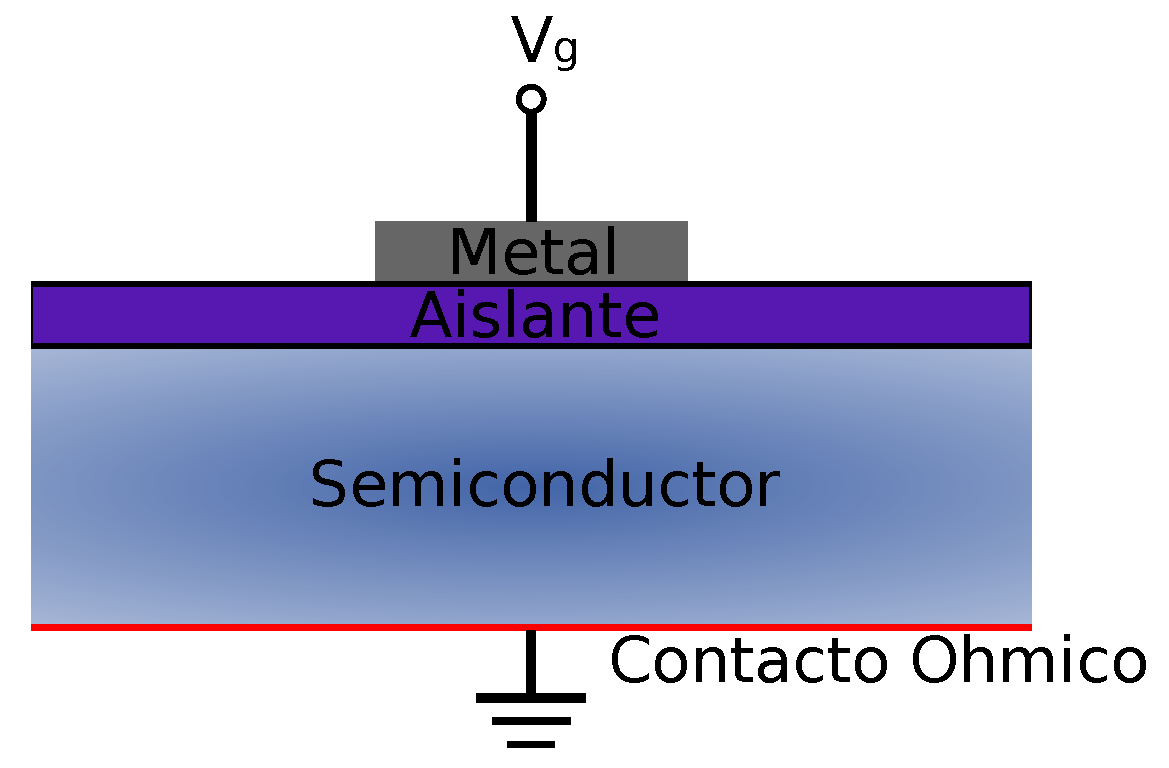
\includegraphics[scale=.35]{Figs/PixelCrossSection.pdf}
    \caption{Esquema de un corte lateral de un capacitor MOS (píxel).}
    \label{fig:PixelCrossSection}
\end{figure}
Además de los píxeles, como se puede ver en la Figura \ref{fig:ArgquitecturaCCDn}, los CCDs están compuestos de \textit{channel-stops} que se encargan de evitar que la carga de los píxeles migre entre columnas vecinas, mientras que los controladores verticales, con las señales $V_{1}$, $V_{2}$ y $V_{3}$, son las responsables de desplazarla secuencialmente de forma vertical. 
Otra parte fundamental de estos detectores es el registro horizontal, donde están los píxeles horizontales de la Figura \ref{fig:ArgquitecturaCCDn}, que es la región del CCD donde la carga es migrada de forma horizontal gracias a los estados $H_{1}$, $H_{2}$ y $H_{3}$ hacia el nodo de sensado.
\begin{figure}[h]
    \centering
        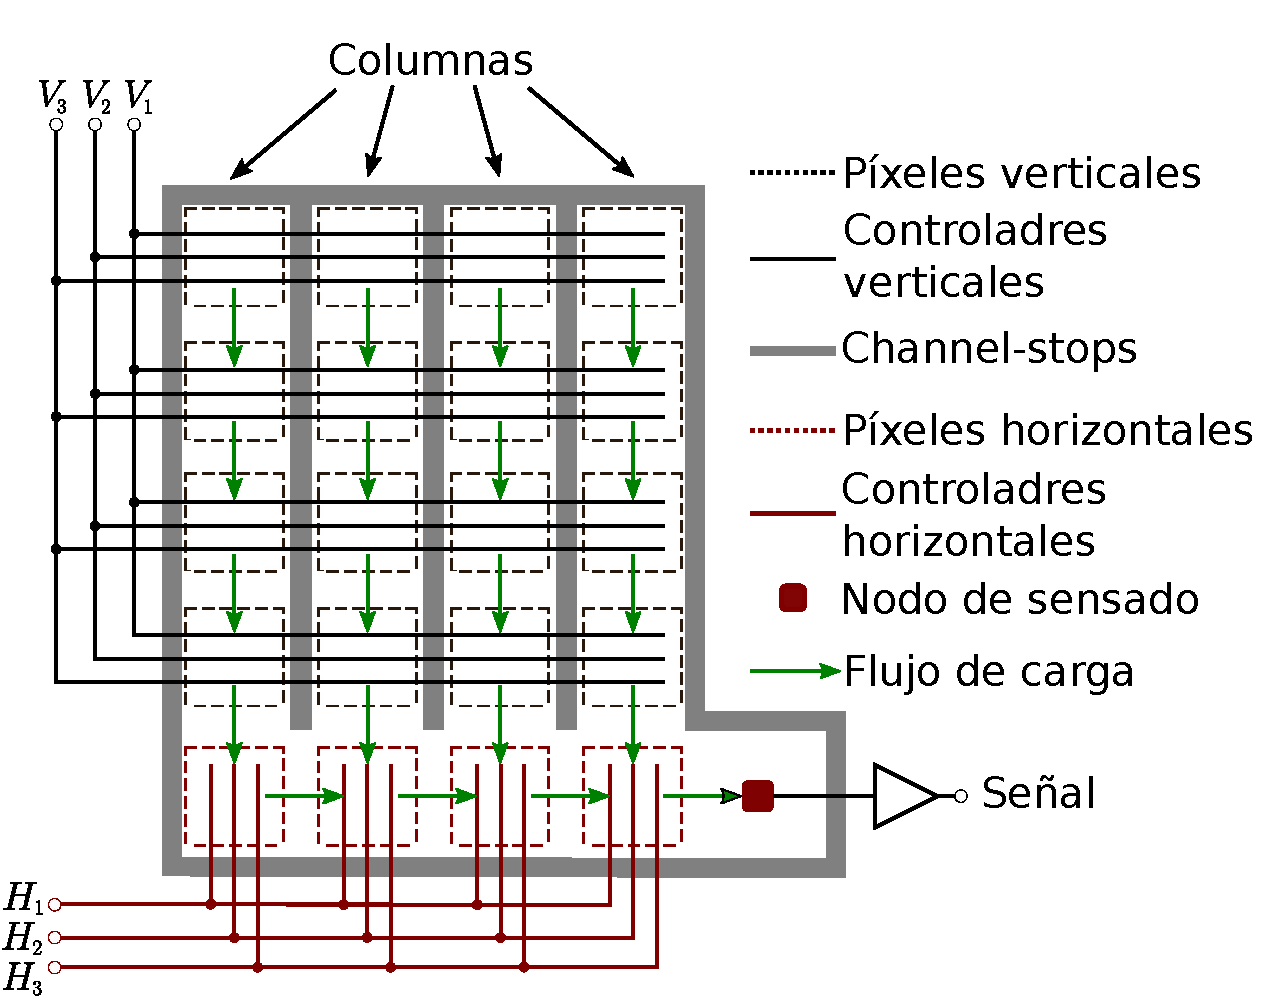
\includegraphics[scale=.5]{Figs/ArquitecturaCCD.pdf}
    \caption{Ilustración esquemática de un sensor CCD de $4\times4$ píxeles. Las flechas muestran la dirección en la que la carga es desplazada píxel a píxel para luego ser colectada por el nodo de sensado.}
    \label{fig:ArgquitecturaCCDn}
\end{figure}
El principio de operación de un CCD se puede dividir en cuatro etapas, que a grandes rasgos son:
\begin{itemize}
    \item Exposición del detector: el tiempo de exposición es variable y depende del tipo de medición que se desee utilizar. Durante la exposición, la radiación incidente interactúa con el detector, generalmente generando pares electrón-hueco. 
    \item Colección: los electrones son luego arrastrados por el campo eléctrico del detector presente en su volumen hacia los pozos de potencial de los píxeles donde son colectados.
    \item Transferencia: dado que la medición de la carga colectada en los píxeles se realiza de forma secuencial, la misma debe ser transferida de un píxel a otro.
    \item Medición de la carga: al llegar al nodo de sensado, un amplificador de salida cuantifica la carga.
\end{itemize}
Los CCD's convencionales son capaces de alcanzar ruidos de lectura del orden de los $2\,e^{-}\si{rms/pix}$, gracias a la técnica de muestreo doblemente correlacionado\cite{Tiffenberg}. Sin embargo, en aplicaciones de bajas energías, el ruido electrónico de lectura redunda en una barrera al límite de energías que pueden medirse con estos sensores manteniendo la precisión deseada. 

Por debajo de los $2\,\si{keV}$ la contribución del ruido de lectura a la determinación del factor de Fano y la energía de creación electrón-hueco puede superar el $30\,\%$, como se esquematiza en la Figura \ref{fig:Fano_y_ruido}. Esto representa un impacto considerable en la determinación de estas cantidades que son de interés en el presente trabajo. La línea punteada en la Figura \ref{fig:Fano_y_ruido} representa el ruido constante de lectura de $30\,\si{eV}$, presente en estos sensores y la recta continua representa el factor de Fano si este fuera constante para todo el rango de energías, tomando $F=0.119$, obtenido experimentalmente y por primera vez para los rayos $X$ del $\Fe{55}$ utilizando la tecnología \textit{skipper}-CCD\cite{Rodrigues}. 
Sobre la curva se ven los puntos que representan los valores del factor de Fano que se medirían si se utilizaran sensores CCD convencionales, debido a la suma de contribuciones del ruido sobre un factor de Fano constante de $0.119$. En la práctica, estas cantidades no están determinadas para el rango de energías inferior a $2\,\si{keV}$ debido a la imposibilidad de medirlas utilizando CCDs convencionales.
\begin{figure}[h]
    \centering
        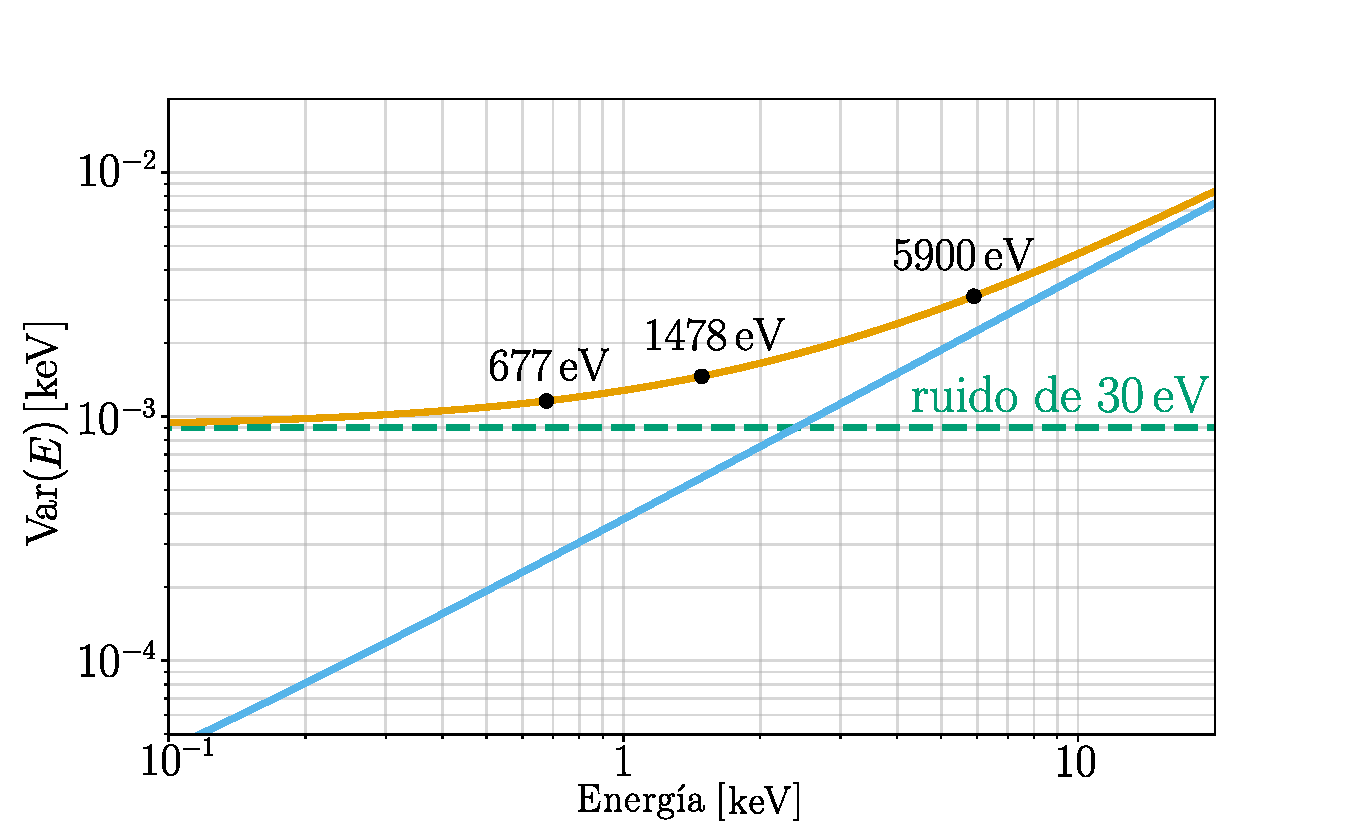
\includegraphics[scale=0.5]{Figs/fano_y_ruido.pdf}
    \caption{Valores que se obtendrían de medir el factor de Fano con un sensor CCD convencional (puntos negros), debido a la contribución del ruido de lectura constante de $30\,\si{eV}$ (línea punteada horizontal). La línea recta de trazo continuo representa un valor de factor de Fano constante de $F = 0.119$.}
    \label{fig:Fano_y_ruido}
\end{figure}

Los sensores \textit{Skipper}-CCD's, por otro lado, permiten disminuir el ruido de lectura a niveles subelectrónicos gracias a que son capaces de medir la carga en los píxeles de forma no destructiva. Esto permite tomar tantas mediciones de la carga como sean necesarias y estimar la carga real a partir de un promedio sobre el número $N$ de mediciones tomadas, de forma que el ruido de lectura se reduce un factor $\sqrt{N}$\cite{Tiffenberg}, es decir, se tiene
\begin{equation*}
    \mu = \frac{1}{N}\sum\limits_{i = 1}^{N} q_{i},
    \quad\quad
    \sigma = \frac{\sigma_{1}}{\sqrt{N}}
\end{equation*}
donde $q_{i}$ es la carga leída en cada proceso de medición y $\sigma_{1}$ es el ruido de lectura para un CCD convencional. 

Esta es la principal razón que motiva este trabajo, donde se realiza un estudio sistemático del factor de Fano a bajas energías, tanto a $1486\,\si{eV}$ (rayos $X$ del Al) y $677\,\si{eV}$ (rayos $X$ del flúor).

%%%%%%%%%%%%%%%%%%%%%%%%%%%%%%%%%%%%%%%%%%%%%%%%%%%%%%%%%%%%%%%%%%
%%%%%%%%%%%%%%%%%%%%%%%%%%%%%%%%%%%%%%%%%%%%%%%%%%%%%%%%%%%%%%%%%%
\section{Modelo de difusión de la carga}
\noindent Dado que el sensor utilizado en este trabajo fue del tipo \textit{back-iluminated}, como se describe en la Sección \ref{subsec:detector}, la mayor parte de las interacciones ocurren en las primeras centenas de nanómetros de la parte trasera del sensor. Con lo cual, para un sensor de $200\,\si{\mu m}$ de espesor, la carga producida durante la ionización debe recorrer prácticamente todo el material hasta alcanzar la superficie donde es colectada. Mientras la carga se transporta desde la parte trasera (cara expuesta) hasta la superficie del detector (cara opuesta a la exposición), ocurre que la carga se difunde desde el píxel donde originalmente fue generada hacia los píxeles vecinos, como se muestra en los esquemas de la Figura \ref{fig:difusion}.
\begin{figure}[h]
    \centering
        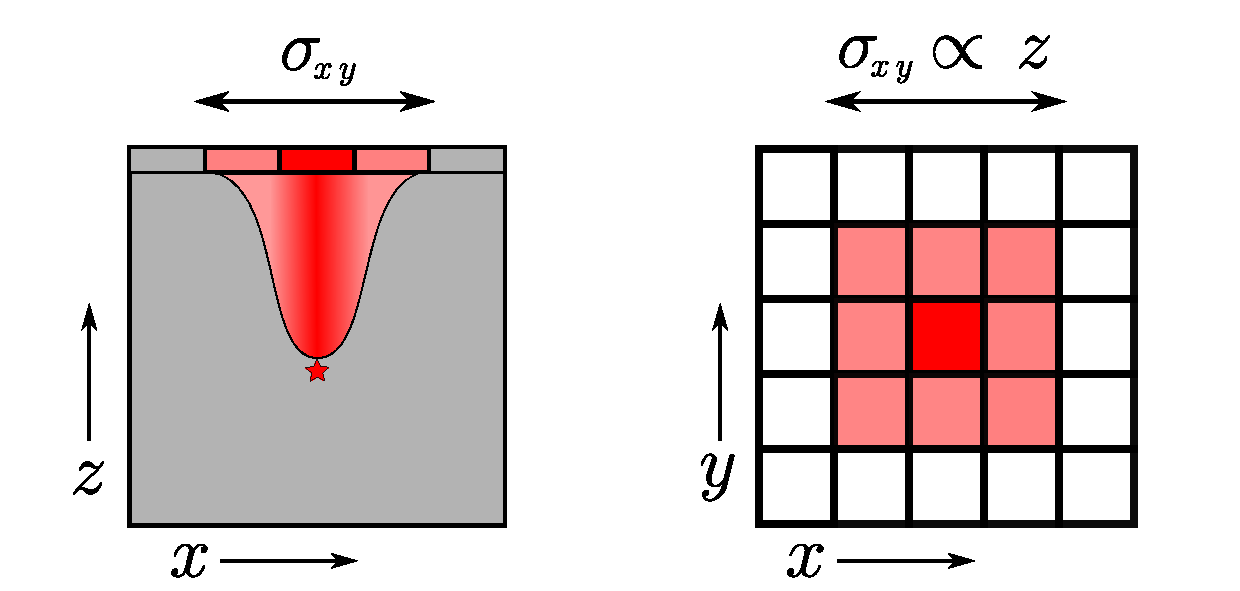
\includegraphics[scale=0.6]{Figs/difusion.pdf}
    \caption{Izquieda: esquematización de la sección transversal de un CCD y de cómo se difunde la carga en los píxeles. Derecha: esquematización frontal de un CCD con la distribución final de la carga sobre un conjunto de píxeles debido a la difusión, denominado cluster. Se colorean más tenues los píxeles representando menor cantidad de carga acumulada.}
    \label{fig:difusion}
\end{figure}
La forma en la que esta difusión ocurre puede modelarse a partir de una distribución gaussiana en dos dimensiones, donde el valor de la varianza $\sigma_{xy}^{2}$ es función de la profundidad $z$ donde ocurrieron las interacciones y se puede escribir como\cite{DifusionCarga}
\begin{equation*}
    \sigma_{xy}^{2} = -A\ln{|1-bz|}
\end{equation*}
donde $A$ y $b$ son parámetros del detector.

Dado que la carga producida por un único evento, inicialmente en un único píxel, puede migrar hacia píxeles vecinos por difusión durante su desplazamiento hacia la superficie, el total de carga producida queda distribuida en varios píxeles contiguos. A este conjunto de píxeles que contiene toda la carga de un único evento se lo denomina cluster.
%%%%%%%%%%%%%%%%%%%%%%%%%%%%%%%%%%%%%%%%%%%%%%%%%%%%%%%%%%%%%%%%%%
%%%%%%%%%%%%%%%%%%%%%%%%%%%%%%%%%%%%%%%%%%%%%%%%%%%%%%%%%%%%%%%%%%
\section{Eficiencia de colección de carga}
\noindent La Eficiencia de Colección de Carga o CCE (\textit{Charge Collection Efficiency}, por sus siglas en inglés) se define como la fracción del total de carga producida durante un evento de ionización que es efectivamente medida. 
Para sensores del tipo \textit{fully depleted}-CCD\cite{osti_838066}, a los que se les aplican campos eléctricos relativamente altos, la CCE es aproximadamente del $100\,\%$, es decir, toda la carga producida por ionización en el volumen del sensor logra ser colectada y medida. 
Sin embargo, existen casos donde la eficiencia no alcanza el $100\,\%$ y esto es debido al fenómeno de Colección Parcial de Carga o PCC (\textit{Partial Charge Collection}, por sus siglas en inglés)\cite{PCC-CCE}. 
Este efecto se debe a que en las primeras centenas de nanómetros cercanos a la superficie por donde se irradia el detector (lado opuesto al que posee la superficie pixelada) existe una probabilidad no nula de que la carga generada por ionización sufra recombinación, es decir, que vuelva a enlazarse a un átomo. Este efecto produce una disminución en el número de cargas que finalmente son llevadas a la superficie del sensor. 
En el esquema de la Figura \ref{fig:PCC} se presenta una vista esquemática en corte lateral de las primeras centenas de nanómetros de un CCD, donde debido al ángulo $\theta$ de incidencia de los rayos $X$ de la fuente, estos fotones generan cargas por ionización en la región donde hay recombinación. Una fracción de las cargas generadas $q_{i}$ logran ser colectadas, dependiendo de la profundidad del sensor donde se produjo la interacción. También se muestra que si la interacción se da fuera de esta región, toda la carga generada por ionización es colectada, teniéndose $q_{i} = q_{f}$ y la eficiencia es máxima.
\begin{figure}%[H]
%Como reproducir este gráfico: correr el script NivelesOcupacionCarga.py ubicado en /Escritorio/Tesis2021/Figs/pys_para_plots y buscar la imagen en /home/igna/Escritorio/Tesis2021/Figs/
    \centering
        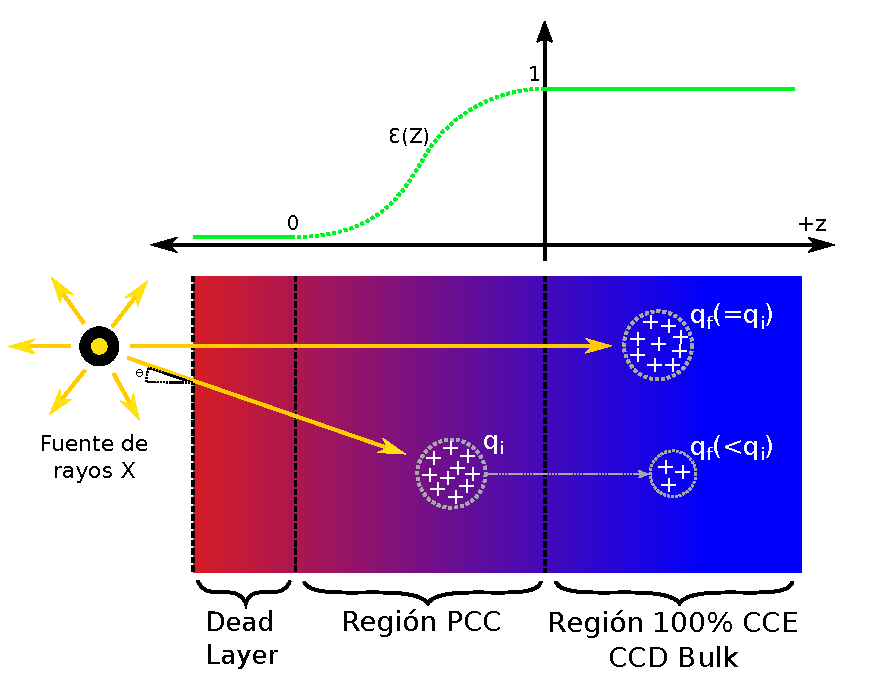
\includegraphics[scale=.8]{Figs/PCC.pdf}
    \caption{Esquema lateral de las primeras centenas de nanómetros de un CCD, con una fuente de rayos $X$\cite{PCC-CCE}. Los fotones penetran en el sensor produciendo una nube de cargas $q_{i}$, de las cuales solo una fracción logra ser colectada. Estas aumentan monótonamente dependiendo de la profundidad de penetración.}
    \label{fig:PCC}
\end{figure}
La colección parcial de carga es un problema propio de los sensores y de su fabricación. Sin embargo, existen tratamientos de la superficie posterior de estos sensores para reducir su impacto y que en general son aplicados en CCDs destinados a toma de imágenes astronómicas. 

El efecto que provoca la colección parcial de carga en las mediciones es el de agregar eventos con menor cantidad de carga de la que deberían, generando así colas a la izquierda de los picos de interés en los espectros y, por ende, agregando otro sesgo a la determinación de magnitudes dependientes del valor medio de los picos, como el factor de Fano.

%%%%%%%%%%%%%%%%%%%%%%%%%%%%%%%%%%%%%%%%%%%%%%%%%%%%%%%%%%%%%%%%%%
%%%%%%%%%%%%%%%%%%%%%%%%%%%%%%%%%%%%%%%%%%%%%%%%%%%%%%%%%%%%%%%%%%

\section{Antecedentes \label{sec:Antecedentes}}
\noindent En trabajos previos se han estudiado las ventajas de la utilización de la tecnología \textit{Skipper} en los CCDs, para lograr medir con precisión subelectrónica en regímenes de energía donde los sensores CCD convencionales más precisos solo podrían alcanzar resoluciones del orden de los $2$ electrones. Por primera vez fue usada para medir el factor de Fano y la energía de creación electrón-hueco en el silicio a una energía de $5.9\,\si{keV}$ a $123\,\si{K}$\cite{Rodrigues}.

Para lograr esto, se implementó un método de calibración absoluta de la relación entre el número de electrones en cada píxel y el valor de lectura en ADUs (\textit{Analog Digital Unit} o Unidades analógico-digitales). El procedimiento para la calibración consistió en la utilización de un LED que emitía fotones en $405\,\si{nm}$ de longitud de onda para poblar de carga los píxeles del sensor. Realizando un barrido en el tiempo de exposición del sensor a la luz del LED, se logró poblar a los píxeles del sensor con un amplio rango de cargas. La medición de carga se realizó tomando $300$ lecturas por cada píxel, que luego fueron promediadas logrando reducir el ruido de lectura en un factor $\sqrt{300}$. Como resultado, se obtuvieron distribuciones de carga gaussianas en los posibles niveles de ocupación de carga con una resolución tal que hizo posible distinguir perfectamente entre picos consecutivos, como se puede ver en la Figura \ref{fig:Calibracion}. De esta forma, mediante un ajuste gaussiano se pudo establecer el valor medio en ADUs para cada uno de estos picos, estableciendo como valor correspondiente de carga el número de orden del pico en cuestión. Así es que se obtuvo una relación uno a uno entre cantidad de carga por píxel y ADUs. Cabe destacar que para comenzar a numerar los picos, primero es necesario establecer el valor de $0$ carga o píxel vacío, lo cual no corresponde, a priori, a un valor nulo en ADUs. Para ello, las imágenes tomadas con \textit{Skipper} cuentan con una región denominada \textit{over-scan} que se utiliza para calcular la línea de base y poder sustraerla luego al valor en ADU medido para cada píxel, logrando así que la media de los píxeles vacíos quede en cero ADUs.
\begin{figure}[H]
%Como reproducir este gráfico: correr el script NivelesOcupacionCarga.py ubicado en /Escritorio/Tesis2021/Figs/pys_para_plots y buscar la imagen en /home/igna/Escritorio/Tesis2021/Figs/
    \centering
        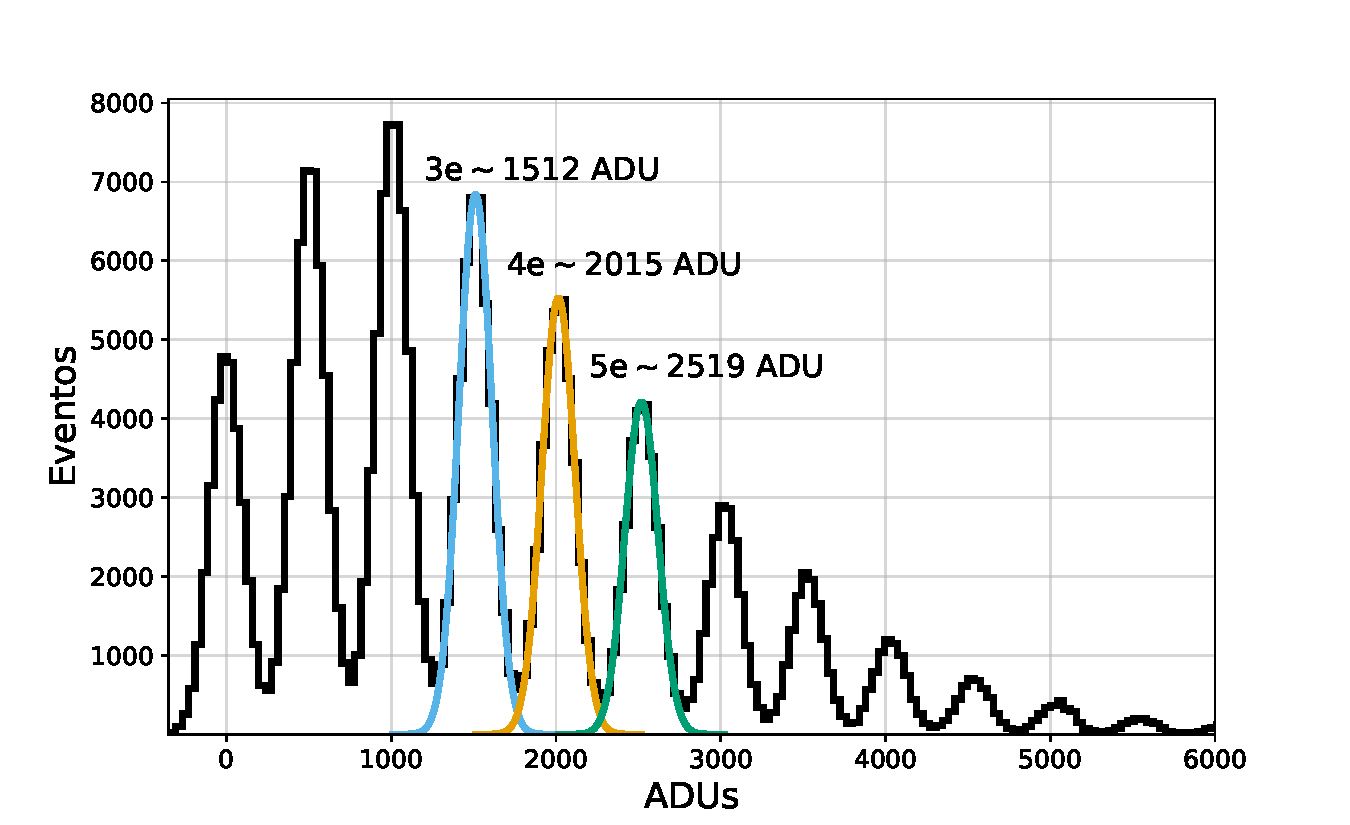
\includegraphics[scale=0.5]{Figs/ajuste_gaussiano_calibracion.pdf}
    \caption{Histograma de los datos obtenidos al iluminar el CCD con LED, correspondiente a una región con poca ocupación, donde los picos de los niveles de carga están ajustados por gaussianas y se distinguen a la perfección.}
    \label{fig:Calibracion}
\end{figure}
Las mediciones del factor de Fano y la energía de creación electrón-hueco se realizaron utilizando rayos $X$ de $5.9\,\si{\mbox{keV}}$ emitidos por una fuente de $\Fe{55}$. Más precisamente, rayos $X_{K}$, cuyas energías son las de la Tabla \ref{tab:EnergiasXk}.
\begin{table}[h]
\centering
\begin{tabular}{@{}ccc@{}}
\toprule
$X_{K}$         &   Energía [eV]   &   Intensidad relativa \\ \hline \hline
$\alpha_{2}$    &   $5887.6$        &   $8.5 (4)$           \\
$\alpha_{1}$    &   $5898.8$        &   $16.9 (8)$          \\
$\beta_{3}$     &   $6490.4$        &   $4.1 (11)$          \\ \bottomrule
\end{tabular}
\caption{Energías e intensidades relativas de los fotones X emitidos tras el decaimiento de $\Fe{55}$}
\label{tab:EnergiasXk}
\end{table}
Sobre los picos de los espectros obtenidos al irradiar el CCD con estos rayos $X$, se realizó un ajuste para obtener los parámetros $\mu$ y $\sigma$ de cada uno. Para esto, se utilizó la verosimilitud de la ecuación \eqref{ec:verosimilitud}, que surge de convolucionar dos distribuciones exponenciales y una distribución gaussiana
{\small
\begin{align}
    \Lagr(e|\mu_{1},
            \mu_{2},
            \sigma_{1},
            \lambda_{1},
            \lambda_{2},
            \eta_{1} = \eta_{2},
            \eta_{3})
    = &
    \sum\limits_{j=1}^{3} I_{j}
    \left\{
        \eta_{j}\frac{\lambda_{1}}{2}
        \exp
            \left[
                (e-\mu_{j})\lambda_{1} + \frac{\sigma_{j}^{2}\lambda_{1}^{2}}{2}
            \right]
        \mbox{Erfc}
        \left[
            \frac{1}{\sqrt{2}}
            \left(
                \frac{e - \mu_{j}}{\sigma_{j}}
                +\sigma_{j}\lambda_{1}
            \right)
        \right] \right. \nonumber
        \\
        + &
        \left.
        (1-\eta_{j})\frac{\lambda_{2}}{2}
        \exp
            \left[
                 (e - \mu_{j})\lambda_{2}
                 + \frac{\sigma_{j}^{2}\lambda_{2}^{2}}{2}
            \right]
        \mbox{Erfc}
        \left[
            \frac{1}{\sqrt{2}}
            \left(
                \frac{e - \mu_{j}}{\sigma_{j}}
                +\sigma_{j}\lambda_{2}
            \right)
        \right]
    \right\}
        \label{ec:verosimilitud}
\end{align}
}%
donde $\mu_{j}$, $\sigma_{j}$ y $I_{j}$ representan el valor medio de carga, la desviación estándar del valor medio de carga y la intensidad relativa del pico $j$-ésimo con energía $E_{j}$, respectivamente y $j = \{\alpha_{1}, \alpha_{2}, \beta_{3}\}$. Además, $\lambda_{1}$ y $\lambda_{2}$ son parámetros de la distribuciones exponenciales y $\eta_{j}$ es el peso relativo entre ellas. Se utilizaron dos exponenciales y una gaussiana para modelar los picos con la intención de describir las colas que había a bajas energías, tomando la descripción que suele hacerse para picos en espectrometría $\alpha$\cite{Bortels}. Sin embargo, se sabe que en este último caso las colas son debidas al fenómeno de auto-absorción, el cual no está presente en los experimentos anteriormente mencionados. Puede decirse entonces que se trató de un modelo fenomenológico, es decir, no basado en primeros principios.
\begin{table}[h]
\centering
\begin{tabular*}{\textwidth}{c @{\extracolsep{\fill}} ccccccccc}%{@{}ccccccccc@{}}
\toprule
$X_{K}$ &
  $\mu\ [e^{-}]$ &
  $\Delta \mu\ [e^{-}]$ &
  $\sigma\ [e^{-}]$ &
  $\Delta \sigma\ [e^{-}]$ &
  $F$ &
  $\Delta F$ &
  $\varepsilon_{\eh}\ [\mbox{eV}]$ &
  $\Delta \varepsilon_{\eh} \ [\mbox{eV}]$ \\ \hline\hline
$\alpha_{2}$ &
  $1570.50$ &
  $0.18$ &
  $13.68$ &
  $0.12$ &
  \multirow{3}{*}{$0.119$} &
  \multirow{3}{*}{$0.002$} &
  \multirow{2}{*}{$3.749$} &
  \multirow{2}{*}{$0.001$} \\
$\alpha_{1}$ & $1573.48$ & $0.18$ & $13.69$ & $0.12$ &  &  &         &         \\
$\beta_{3}$  & $1730.50$ & $0.55$ & $14.36$ & $0.13$ &  &  & $3.751$ & $0.002$ \\ \bottomrule
\end{tabular*}
\caption{Parámetros obtenidos de los ajustes para las mediciones del $\Fe{55}$. El factor de Fano se tomó el mismo para los tres picos y la energía de creación electrón-hueco se fijó para que sea la misma en los picos $\alpha$.}
\label{tab:ParametrosAjusteNoBineado}
\end{table}

Así es que los valores condensados en la Tabla \ref{tab:ParametrosAjusteNoBineado} constituyen los primeros resultados obtenidos de la utilización de la tecnología \textit{Skipper}-CCD para el cálculo del factor de Fano y de la energía de creación electrón-hueco para una temperatura de $123\,\si{K}$. Los mismos se encuentran en excelente acuerdo con la bibliografía preexistente~\cite{Ryan, Alig, Kotov} y presentan la mejor incerteza alcanzada a la fecha.

En esa oportunidad se llevaron a cabo además las primeras mediciones tendientes a determinar el factor de Fano y la energía de creación electrón-hueco para energías por debajo de los de $2\,\si{keV}$~\cite{TesisKevin}, más específicamente, para energías de $677\,\si{eV}$ y $1486\,\si{eV}$, que corresponden a los rayos $X$ de fluorescencia del flúor y del aluminio respectivamente. En la Tabla \ref{tab:EnergiasFluorescenciaFAl} pueden verse las energías e intensidades relativas para los rayos $X$ de estos elementos. Esto se logró a partir de mediciones realizadas con una fuente de $\Am{241}$ que emite partículas $\alpha$ con una energía de $\sim 5.6\,\si{MeV}$. A estas partículas se las hizo impactar contra una cinta de teflón (que contiene flúor) y una barra de aluminio que por fluorescencia emitían rayos $X$ con las energías antes mencionadas. 
\begin{table}[h]
\centering
\begin{tabular}{@{}cccc@{}}
\toprule
Elemento    &   $X_{K}$         &   Energía [eV]    &   Intensidad relativa \\ \hline \hline
F           &   $\alpha_{1,2}$  &   $676.8$         &   $148$               \\
Al          &   $\alpha_{2}$    &   $1486.3$        &   $50$                \\
Al          &   $\alpha_{1}$    &   $1486.7$        &   $100$               \\
Al          &   $\beta_{1}$     &   $1557.4$        &   $1$                 \\ \bottomrule
\end{tabular}
\caption{Energías e intensidades de las líneas de emisión de rayos $X$ para el flúor y el aluminio en el rango de energías por debajo de los $2\,\si{keV}$.}
\label{tab:EnergiasFluorescenciaFAl}
\end{table}

Uno de los desafíos que surgieron en este otro trabajo fue obtener una buena estadística, debido a que solo una fracción muy pequeña de los átomos que son impactados por las partículas $\alpha$ se desexcitan emitiendo fotones $X$ en las energías de deseadas. La emisión de rayos $X$ tras la captura electrónica del núcleo del $\Fe{55}$, en cambio, ocurre siempre y por lo tanto es proporcional a la actividad de la fuente. Por esta razón, dada una misma actividad de la fuente de $\Fe{55}$ y la tasa de emisión de partículas $\alpha$, la obtención de rayos $X$ es mucho más probable en el primer caso, haciendo la colección de eventos más rápida.

Con los datos de estas mediciones se reconstruyeron los espectros para ambos picos y se les realizó un ajuste muy similar al de los experimentos con $\Fe{55}$, utilizando la verosimilitud descripta por la expresión \eqref{ec:verosimilitudF-Al}
\begin{align}
    \Lagr(e|\mu,
            \sigma,
            \lambda_{1},
            \lambda_{2},
            \eta)
    = &
    \eta
    \left\{
        \frac{\lambda_{1}}{2}
        \exp\left[
                (e-\mu)\lambda_{1} + \frac{\sigma^{2}\lambda_{1}^{2}}{2}
            \right]
        \mbox{Erfc}
        \left[
            \frac{1}{\sqrt{2}}
            \left(
                \frac{e - \mu}{\sigma}
                +\sigma\lambda_{1}
            \right)
        \right] \right\} \nonumber
        \\
        + &
        (1-\eta)
        \left\{
        \frac{\lambda_{2}}{2}
        \exp
            \left[
                 (e - \mu)\lambda_{2}
                 + \frac{\sigma^{2}\lambda_{2}^{2}}{2}
            \right]
        \mbox{Erfc}
        \left[
            \frac{1}{\sqrt{2}}
            \left(
                \frac{e - \mu}{\sigma}
                +\sigma\lambda_{2}
            \right)
        \right]
    \right\}
        \label{ec:verosimilitudF-Al}
\end{align}

Los resultados obtenidos en este trabajo se encuentran en la Tabla \ref{tab:ParametrosAjusteNoBineadoF-Al}.
\begin{table}[h]
\centering
\begin{tabular*}{\textwidth}{c @{\extracolsep{\fill}} ccccccccc}%{@{}ccccccccc@{}}
\toprule
Elemento&
  $\mu\ [e^{-}]$ &
  $\Delta \mu\ [e^{-}]$ &
  $\sigma\ [e^{-}]$ &
  $\Delta \sigma\ [e^{-}]$ &
  $F$ &
  $\Delta F$ &
  $\varepsilon_{\eh}\ [\mbox{eV}]$ &
  $\Delta \varepsilon_{\eh} \ [\mbox{eV}]$ \\ \hline\hline
  F &   $182.0$ &   $0.8$  &   $7.0$   &   $0.7$   &   $0.27$  &   $0.05$  &   $3.72$ &   $0.02$\\
  Al&   $404.4$ &   $0.4$  &   $8.3$   &   $0.3$   &   $0.17$  &   $0.01$  &   $3.679$ &   $0.004$\\ \bottomrule
\end{tabular*}
\caption{Resultados preliminares obtenidos en un trabajo previo para el factor de Fano y la energía de creación electrón-hueco para las energías de los rayos $X$ de fluorescencia del flúor y el aluminio.}
\label{tab:ParametrosAjusteNoBineadoF-Al}
\end{table}

Sin embargo, estos últimos fueron resultados preliminares que podían mejorarse tanto aumentando la estadística, como realizando un análisis de los datos más sofisticado. Sobre este último punto, vale decir que el modelo de ajuste utilizado antes de esta tesis no incluye los efectos de la colección parcial de carga. Además, en el análisis de las imágenes, no se realizó ninguna corrección por el sesgo que podría significar la adición de carga originada por fuentes de fondo descriptas en la próxima sección.

Es a partir de aquí donde este trabajo continúa con el estudio del factor de Fano, la energía de creación electrón-hueco y la colección parcial de carga, a partir de mediciones de rayos X con energías por debajo de los $2\,\si{keV}$.

%%%%%%%%%%%%%%%%%%%%%%%%%%%%%%%%%%%%%%%%%%%%%%%%%%%%%%%%%%%%%%%%%%
%%%%%%%%%%%%%%%%%%%%%%%%%%%%%%%%%%%%%%%%%%%%%%%%%%%%%%%%%%%%%%%%%%
\section{Motivación del análisis de imágenes}
\noindent El fondo presente en las imágenes tiene diferentes orígenes, uno de ellos es la carga producida por fluctuaciones térmicas en la red cristalina del silicio del sensor (corrientes oscuras). Otra contribución es la de eventos de dispersión Compton, producidos por la interacción de los fotones con los materiales que rodean al sensor y también en la red cristalina del mismo. Podemos incluir además, aquellos fotones infrarrojos emitidos desde los materiales que rodean al detector cuando estos son excitados por radiación circundante o bien por radiación de cuerpo negro. También se encuentran los eventos de carga producida por radiación muy penetrante provenientes del exterior, como por ejemplo, muones.

Parte del análisis consistió en estudiar el efecto que produce el fondo de las imágenes sobre los eventos de interés: la aglomeración de píxeles con un único electrón alrededor de los clusters, y la carga extra añadida sobre ellos. 
En muchos casos resulta que los píxeles con fondo se aglutinan a los clusters, aumentando su tamaño y su carga, o incluso también haciendo de puente entre dos clusters vecinos. Estos son dos efectos indeseados, primero, porque sesgan la cantidad de carga real en un evento y segundo, porque los programas de reconocimiento de eventos podrían ignorarlos al no cumplir con los cortes de calidad impuestos\footnote{Ver sección \ref{sec:ProcesadoDatos}}, tanto por forma como por cantidad de carga, produciendo así una disminución en la estadística.

En este contexto, se propone utilizar un umbral de detección que ignore píxeles con un solo electrón, de forma de evitar el agregado de píxeles con una carga inducida por eventos de fondo a los clusters y con este corte lograr aumentar la estadística en el conteo de eventos. Para ello, también es necesario lograr caracterizar el fondo responsable de este efecto para corregir el sesgo introducido por el nuevo umbral de detección, el cual también eliminará píxeles con una carga genuina.
%
Es por eso que en este trabajo se desea realizar un análisis de las imágenes del cual obtener un método que pueda corregir el sesgo introducido luego de recuperar la mayor estadística posible separando eventos unidos por un electrón de fondo. 
Esto es, el desarrollo de un método para estimar en valores medios cuántos electrones genuinos son removidos y cuántos electrones de fondo hay en los clusters, para eliminar así sesgos y eventualmente reducir además las incertezas en la determinación del factor de Fano y la energía de creación electrón-hueco a bajas energías.

Motiva también este trabajo el desarrollo y aplicación de un modelo que permita dar cuenta del efecto de colección parcial de carga y así obtener una forma analítica para la distribución de carga producida por los fotones de interés.

%%%%%%%%%%%%%%%%%%%%%%%%%%%%%%%%%%%%%%%%%%%%%%%%%%%%%%%%%%%%%%%%%%
%%%%%%%%%%%%%%%%%%%%%%%%%%%%%%%%%%%%%%%%%%%%%%%%%%%%%%%%%%%%%%%%%%
\section{Organización de la tesis}
\noindent En el presente capítulo se ha dado una breve introducción a los tres aspectos principales de estudio de este trabajo: el factor de Fano, la energía de creación electrón-hueco y la colección parcial de carga. Además se han presentado resultados que conforman los antecedentes para la motivación de esta tesis.

En el capítulo \ref{chap:simulaciones} se presenta un modelo físico simple de la interacción entre fotones incidentes y la red cristalina del sensor, que luego es utilizado en simulaciones Monte Carlo tendientes a reproducir los valores experimentalmente observados para el Factor de Fano.

En el capítulo \ref{chap:ConfiguracionExperimental} se desarrolla una descripción esquemática del dispositivo de medición utilizado y los regímenes de trabajo necesarios para su correcta operación. También se da una breve descripción del sensor y de los materiales que lo componen, como así también de la fuente radioactiva utilizada. Por último, se describe el proceso de medición.

En el capítulo \ref{chap:Analisis} se describe cómo son procesados los datos y qué programas son utilizados además de las pruebas realizadas con distintos umbrales para la detección de carga. También se muestran los resultados del análisis realizado para caracterizar el sensor. Es en este capítulo que se describen los diferentes enfoques utilizados en la estimación del fondo y de la cantidad de eventos eliminados por el umbral de detección de carga (corte) utilizado y el método aplicado para realizar las correcciones sobre el sesgo sobre carga de cada evento introducido por el corte aplicado.

En el capítulo \ref{chap:ModeloPCC} se introduce un modelo que describe la distribución de carga considerando no solo el factor de Fano sino además el efecto que la colección parcial de carga tiene sobre las distribuciones de carga estudiadas.

Por último, en el capítulo \ref{chap:Resultados} se presentan los resultados obtenidos para el Factor de Fano, la energía de creación electrón-hueco y el ancho efectivo de la zona de colección parcial de carga, a partir de ajustes no bineados sobre los espectros de carga medidos y utilizando el modelo descripto en el Capítulo \ref{chap:ModeloPCC}.

